\begin{samepage}
\begin{lstlisting}[language=xml,label=lst:background:apis:soap-request,caption={[An example SOAP request]A \gls{soap} \glsac{http} POST consumer request to retrieve customer record \#43456 from a web service provider. Source: \citep{Ballinger:2014aa}.}]
POST /customers HTTP/1.1
Host: www.example.org
Content-Type: application/soap+xml; charset=utf-8

<?xml version="1.0"?>
<soap:Envelope 
  xmlns:soap="http://www.w3.org/2003/05/soap-envelope">
  <soap:Body>
    <m:GetCustomer 
      xmlns:m="http://www.example.org/customers">
      <m:CustomerId>43456</m:CustomerId>
    </m:GetCustomer>
  </soap:Body>
</soap:Envelope>
\end{lstlisting}
\begin{lstlisting}[language=xml,label=lst:background:apis:soap-response,caption={[An example SOAP response]The \gls{soap} \glsac{http} service provider response for \cref{lst:background:apis:soap-request}. Source: \citep{Ballinger:2014aa}.}]
HTTP/1.1 200 OK
Content-Type: application/soap+xml; charset=utf-8

<?xml version='1.0' ?>
<env:Envelope 
  xmlns:env="http://www.w3.org/2003/05/soap-envelope" >
  <env:Body>
    <m:GetCustomerResponse 
      xmlns:m="http://www.example.org/customers">
      <m:Customer>Foobar Quux, inc</m:Customer>
    </m:GetCustomerResponse>
  </env:Body>
</env:Envelope>
\end{lstlisting}
\end{samepage}

\newpage
\begin{samepage}
\begin{lstlisting}[label=lst:background:apis:rest-request,caption={[An example RESTful request]An equivalent \glsac{http} consumer request to that of \cref{lst:background:apis:soap-request}, but using \gls{rest}. Source: \citep{Ballinger:2014aa}.}]
GET /customers/43456 HTTP/1.1
Host: www.example.org
\end{lstlisting}
\begin{lstlisting}[language=json,label=lst:background:apis:rest-response,caption={[An example RESTful response]The \gls{rest} \glsac{http} service provider response for \cref{lst:background:apis:rest-request}. Source: \citep{Ballinger:2014aa}.}]
HTTP/1.1 200 OK
Content-Type: application/json; charset=utf-8

{"Customer": "Foobar Quux, inc"}
\end{lstlisting}
\end{samepage}

\begin{figure}[p!]
\centering
\caption[Categorisation of AI-based products and services]{A Broad Range of \gls{ai}-Based Products And Services Is Already Visible. (From \citep{LoGiudice:2016wf}.)}
\label{fig:introduction:ai-products}
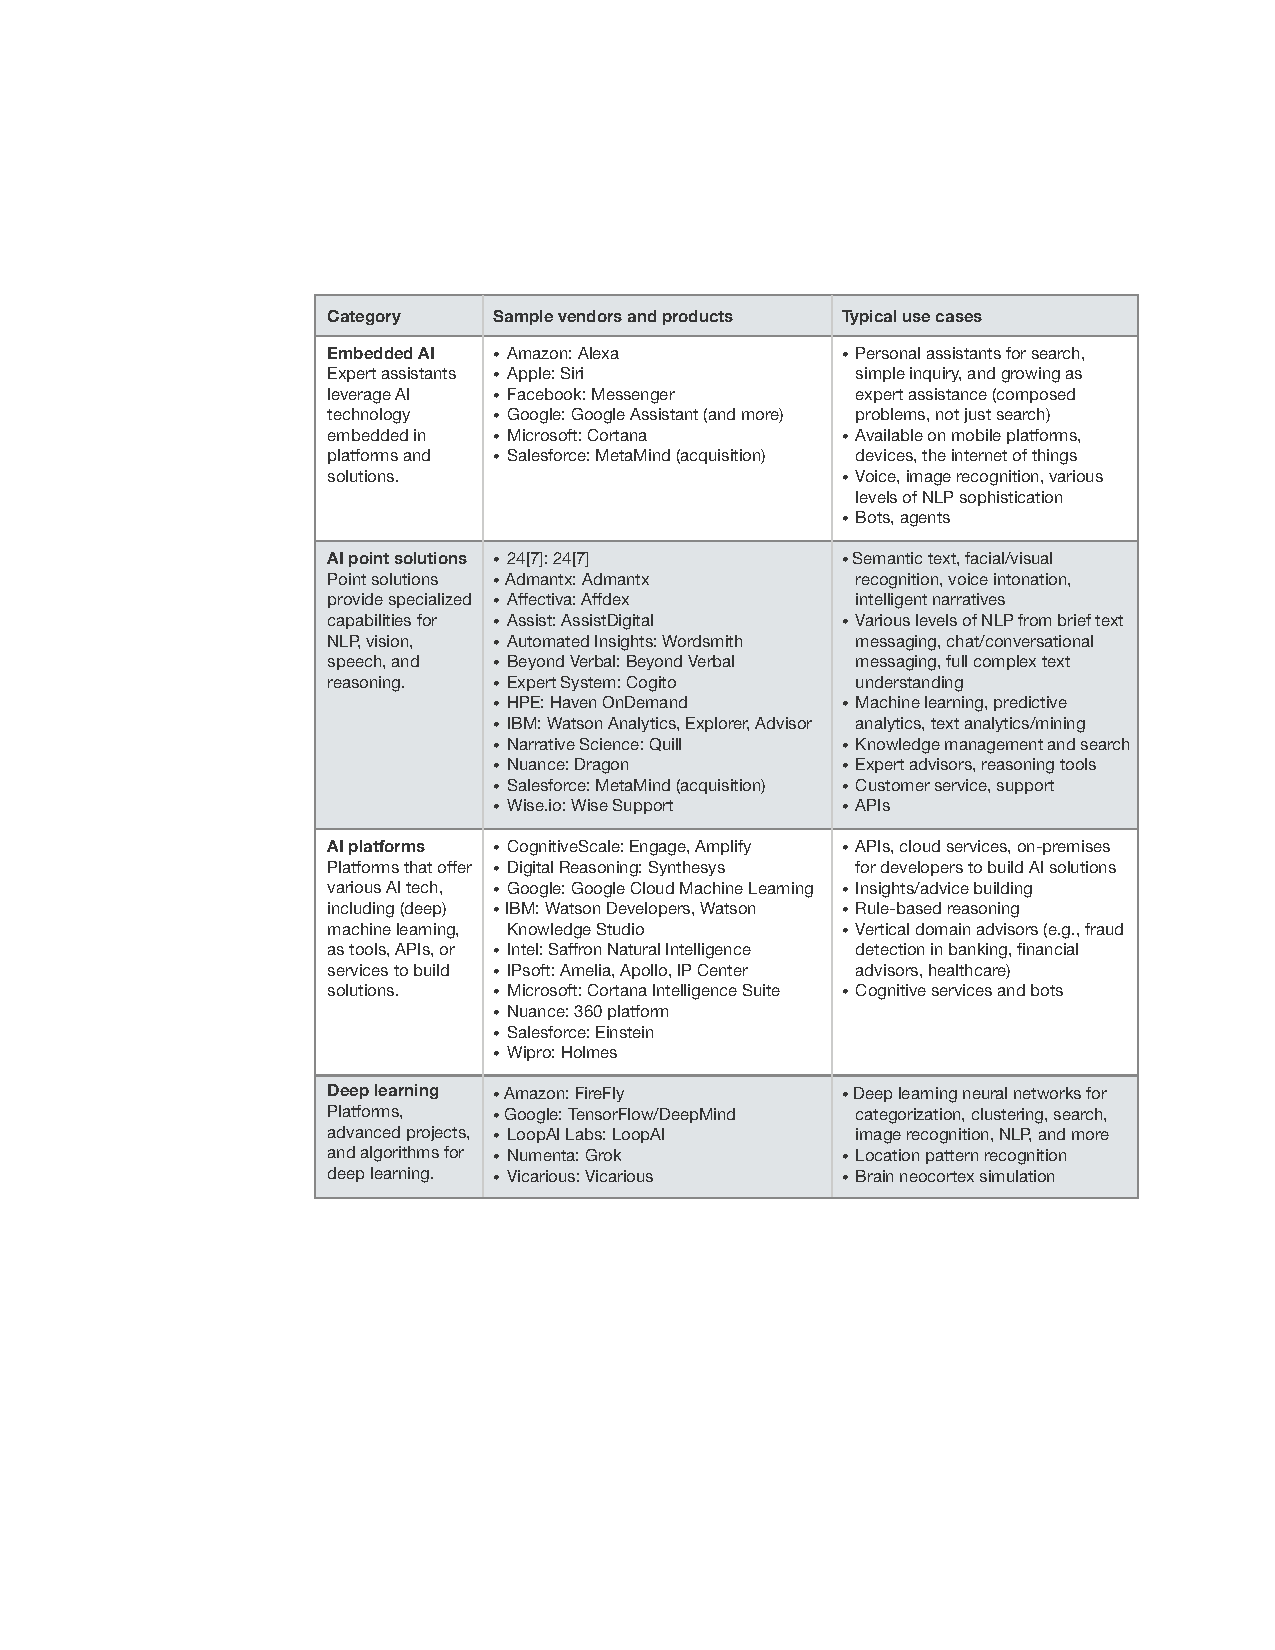
\includegraphics[width=\linewidth]{mainmatter/introduction/figures/ai-products}
\end{figure}

\begin{figure}[p!]
\centering
\caption[Increasing interest in the developer community of computer vision APIs]{Increasing interest on Stack Overflow for these intelligent cloud services.}
\label{fig:introduction:stackoverflow-trends}
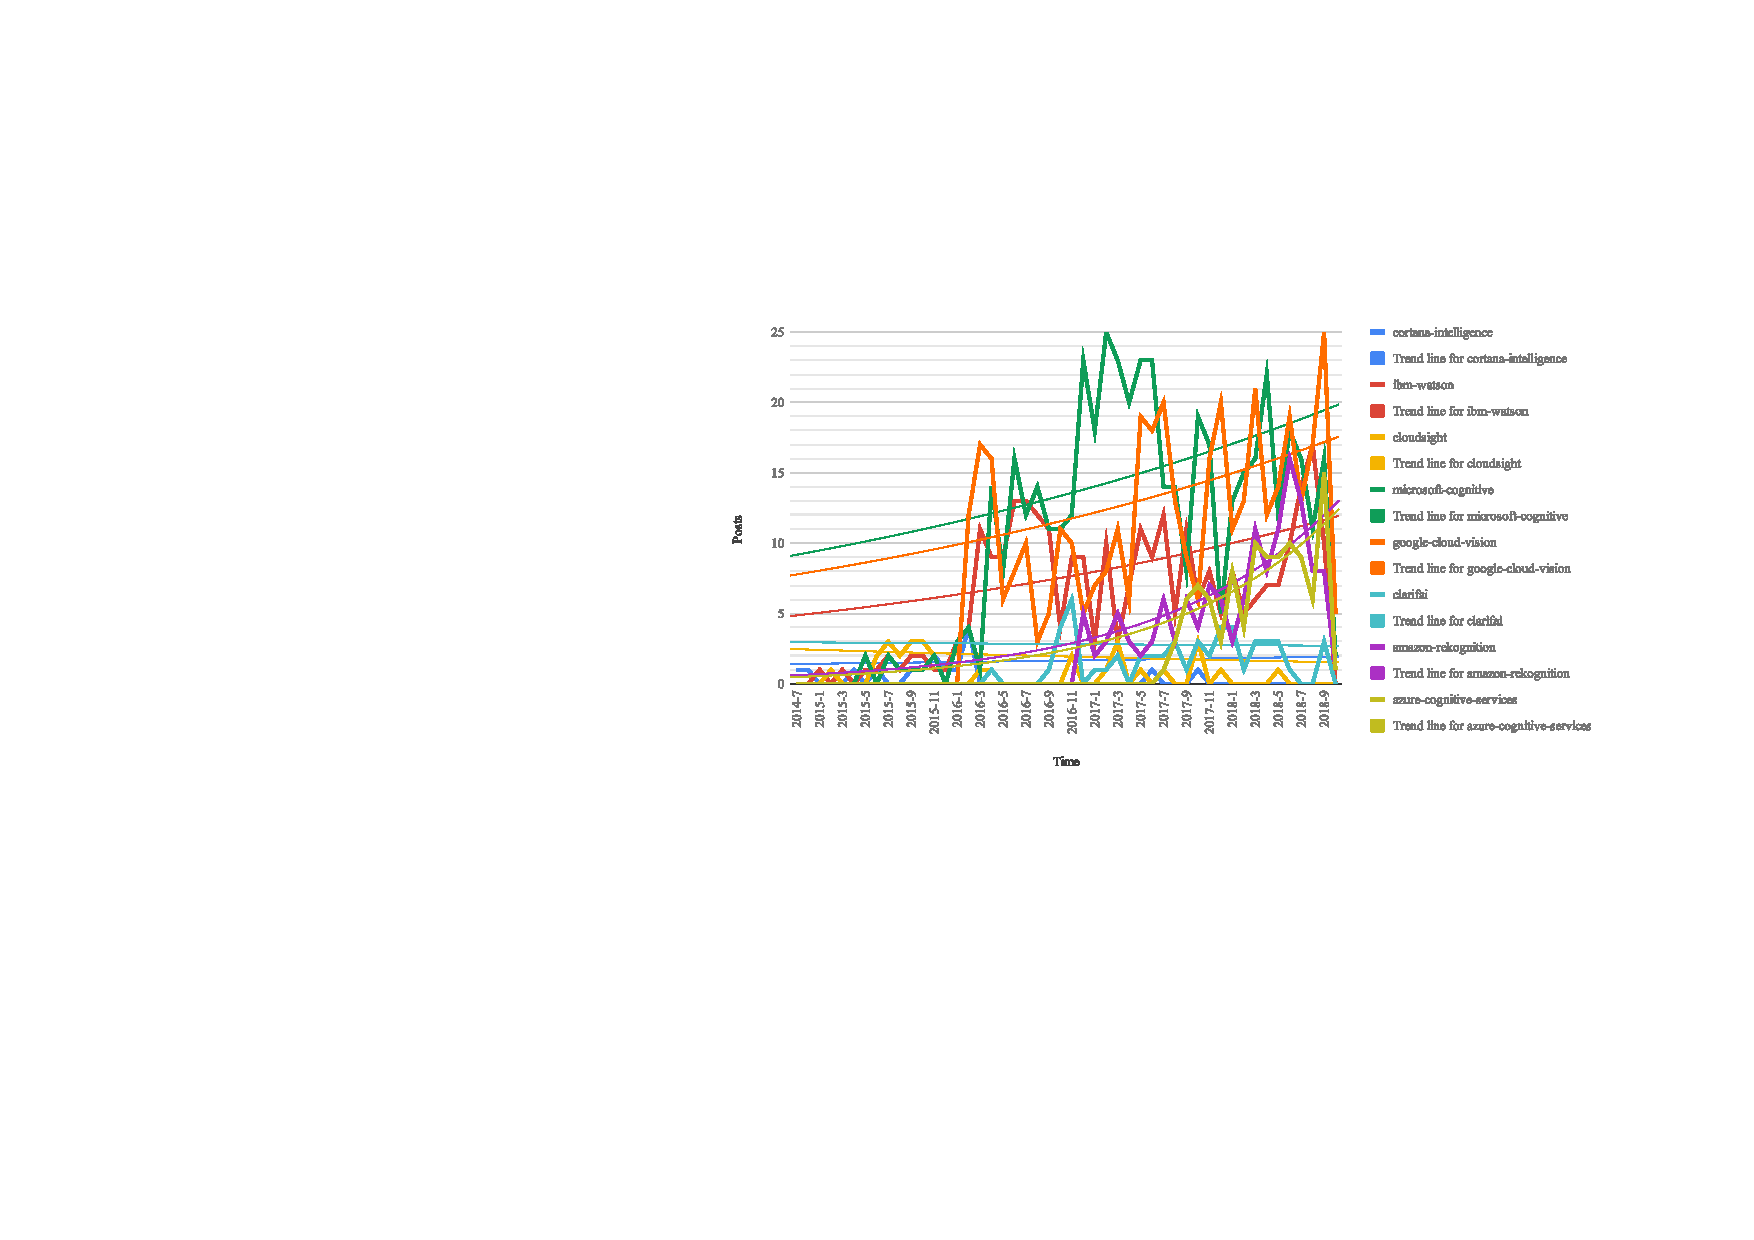
\includegraphics{mainmatter/introduction/figures/stackoverflow-trends}
\end{figure}

\begin{figure}[p!]
\centering
\caption[Review of field study techniques]{Questions asked by software engineering researchers (column 2) that can be answered by field study techniques. (From \citep{Singer:2007tu}.)}
\label{fig:research-methodology:review:field-techniques}
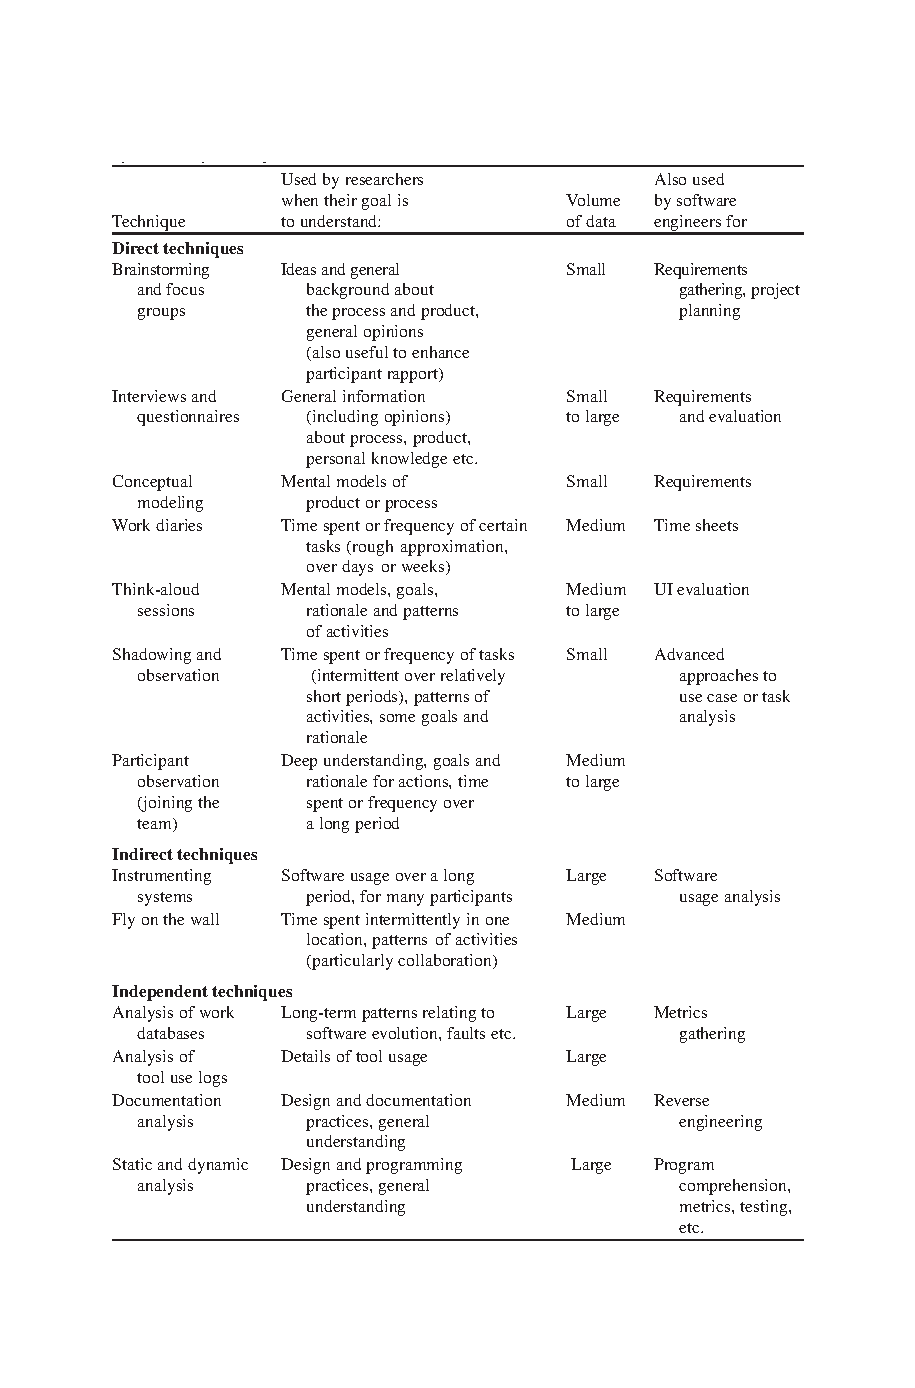
\includegraphics[width=0.95\linewidth]{mainmatter/research-methodology/figures/field-techniques}
\end{figure}